\documentclass{mai_book}

\defaultfontfeatures{Mapping=tex-text}
\setmainfont{DejaVuSerif}
\setdefaultlanguage{russian}

\begin{document}

%\lhead{\small\textit{Упражнений}}
%\rhead{387}%

\noindent {\bf that, as she goes round the court, she may always find the number in each sty
nearer to ten than the number in the last."

“Does she call ten nearer to ten than nine is?” said Norman.

“Surely," said the Governor. "Her Radiancy would adm it th at ten is nearer
to ten than nine is—and also nearer than eleven is."

“Then I think it can be done," said Norman\footnote{%
{\small — Он в глубоком отчаянии, — пояснил губернатор, когда наши путешествен-
ники покинули плац.

— Ее Блистательство повелела ему разместить в четырех угловых свинарниках
24 поросенка так, чтобы при обходе плаца число поросят в очередном свинарнике
неизменно оказывалось ближе к 10, чем число поросят в предыдущем.

— Считает ли Ее Блистательство, что 10 ближе к 10, чем 9? — спросил Норман.

— О да! — подтвердил губернатор. — Ее Блистательство не только считает, что
10 ближе к 10, чем 9, но и выражает уверенность в том, что 10 ближе к 10, чем 11.

— Тогда, я полагаю, поросят можно разместить требуемым образом, — сказал
Норман.

(Перевод Ю. А. Данилова, Л. Кэррол «История с узелками», М., Мир, 1973.)}
}}...

\newpage
\cleartop

\begin{center}
{\par\bigskip{\LARGE \bf Решение упражнений}}
\end{center}

\paragraph{1. Евклидовы возрастающие алгоритмы}

\subparagraph{a и c.} Смотрите упражнения 12 и 13 главы II.

\subparagraph{b.} Пусть $a = bq + r$ евклидово деление $a$ на $b$. Так как $b$ делит $a$,
$b$ также делит $r$; и если предположить, что $r$ не нуль, то $(\varphi(b) \leqslant (\varphi(r)$
(в силу возрастания $\varphi$) и $\varphi(r) < \varphi(b)$ (так как $a = bq + r$ --- евклидово
деление). Получили противоречие. Следовательно, $r$ нуль.

\paragraph{2. Явное выражение подмодуля}

\subparagraph{a.} Модуль $A^{n}$ нётеров, и следовательно, любой подмодуль порожден
конечным числом векторов. Если $E \subset A^{n}$ представимо в виде Ker\,{$X$},
где $X$ --- матрица с элементами в $A$, то $\lambda{x} \in E$, где $\lambda \neq 0$, влечет
принадлежность $x \in E$. Естественно, существует подмодуль, не удо-
влетворяющий этому свойству. Теория модулей над кольцами главных
идеалов состоит, в частности, в представлении в общем виде подмоду-
лей из $A^{n}$.

\subparagraph{b.} Существует сюръекция из $A^{m}$ на модуль в вопросе...

\subparagraph{c.} Пусть $X, Y, Z$,... --- матрицы подходящих размеров. Следую-
щие выражения являются явным представлением модулей: Im\,{$X$}, Кеr\,{$X$},
Im\,{$X$} $\cap$ Im\,{$Y$}, $Z$(Im\,{$X$}), $Z^{-1}$({Im\,{$Y$}) и др.

\paragraph{3. Система образующих для $\rm{SL_{2}}(\mathbb {Z})$}

\subparagraph{\bf a.} Имеют место соотношения:

\begin{gather*}
A^{2} = -I,\;\;\;A^{4} = I,\;\;\;B_{q}B_{q'} = B_{q+q'}, \\
B^{-1}_{q} = B_{-q},\;\;\;C_{q} = AB_{q},\;\;\;C = AB^{-1},\;\;\;C^{3} = I.  \notag
\end{gather*}

\noindent Кроме того, $B_{q} = B^{q}$ и $B$ конечного порядка.

\subparagraph{b.} Евклидово деление $a$ на $b$ может быть записано в следующем виде:
$b' = a + bq$, где $|b'| < |b|$, a $q$ --- искомое.


\restoretop
\newtopre{III Модули над кольцами главных идеалов}
\newtoplo{Решение упражнений}
%\lhead{\small{\it Решение упражнений}}
%\rhead{389}

\subparagraph{c.} Пусть $a, b, c, d$ элементы матрицы из $\rm{SL_{2}}(\mathbb {Z})$. В силу пункта {\bf b} рассмотрим подходящую матрицу $M$. Так как матрицы имеют определители 1, то можно записать:

\begin{equation*}
M\;\;{\begin{pmatrix} a & c \\ b & d \end{pmatrix}} = \begin{pmatrix} 1 & q \\ 0 & 1 \end{pmatrix} = B^{q}\;\;\;\;\;\;\text{или}\;\;\;\;\;\;M\;\;{\begin{pmatrix} a & c \\ b & d \end{pmatrix}} = \begin{pmatrix} -1 & -q \\ 0 & -1 \end{pmatrix} = A^{2}B^{q},
\end{equation*}

\noindent что доказывает тот факт, что $\rm{SL_{2}}(\mathbb{Z})$ порожден $A$ и $B$ (и конечно, $A$ и $C$).

\paragraph{4. Метод приведения к ступенчатому виду для вектора} \mbox{}\\

Метод дает скаляр $d$ и обратимую $m \times m$-матрицу $R$, удовлетворя ющие условию:

\begin{equation*}
(d,0,0,\ldots,0) = (x_1,х_2,х_3,\ldots,x_m) \times R,
\end{equation*}

\noindent и следовательно, $Ad = Ax_1 + Ax_2 +\ldots+ Ax_{m}$; $d$ является наибольшим общим делителем $x_{i}$, а первый столбец $R$ дает коэффициенты Безу.

\paragraph{5. Необходимое и достаточное условие того, что $Ax$ является
\;\;\;прямым слагаемым в $A^{n}$}

\subparagraph{a.} Если $f_1,f_2,\ldots,f_n$ - базис $A^{n}$, где $f_1 = x$, то линейная форма $g$, проекция на $f_1$, т.е. определенная равенством $g(\sum_{i=1}^{n} \lambda_{i}f_{i}) = \lambda_{1}$, удовлетворяет условию $g(x)$ = 1. Применив отношение Безу $\sum_{i=1}^{n} x_{i}g(e_{i})$ = 1, доказываем, что координаты $x_i$, вектора $x$ попарно взаимно просты.

Обратно, если координаты взаимно просты, применим равенство Безу: $\sum_{i=1}^{n} u_{i}x_{i}$ = 1, которое позволяет определить линейную форму $g$ (через равенство $g(y) = \sum_{i=1}^{n} u_{i}y_{i}$), удовлетворяющую условию $g(x)$ = 1. Рассмотрим разложение $A^n = Ax \oplus Ker{g}$ (пишут $y = \lambda{x} + (y — \lambda{x})$ и выражают $\lambda$, чтобы $g(y — \lambda{x})$ = 0). Достаточно рассмотреть базис \{$f_2,f_3,\ldots,f_n$\} Ker\,{$g$}.

\begin{wrapfigure}{r}{5cm}
\begin{equation*}
R = \begin{pmatrix} -1 & 2 & 1 & 1 \\ 1 & -3 & -1 & -1 \\ 0 & 0 & 1 & 0 \\ 0 & 0 & 0 & 1 \end{pmatrix}
\end{equation*}
\end{wrapfigure}
\subparagraph{b.} Можно определить коэффициенты
Безу, и как следствие, линейную форму $g$,
а значит, можно выразить базис Кег\,{$g$}. На-
пример, для $g$ = (30,42,70,105) можно
взять следующую линейную форму:

\begin{equation*}
g(y) = -3y_1 - 2y_2 + y_3 + y_4.
\end{equation*}

\noindent Она будет удовлетворять условию $g(x)$ = 1. Алгоритм приведения к ступенчатому виду, примененный к матрице $g$ = (—3,-2,1,1), дает обратимую матрицу $R$, три последних столбца которой образуют базис Ker{$g$}. Эти три столбца и вектор $x$ образуют базис $\mathbb {Z}^{4}$.



%\lhead{390}
%\rhead{\small\textit{\rm{III} Модули над кольцами главных идеалов}}

\paragraph{6. Определители и линейная независимость\\
над коммутативным кольцом}

\subparagraph{a.} Достаточно разложить по первой строке определитель поряд-
ка $m$, образованный из столбцов векторов $p_{J}v_{i}$, ограниченный свер-
ху строкой $(p_{j}v_{1},\ldots,p_{j}v_{m})$. Как только эта строка появится в ниж-
ней части этого определителя, то результат будет равен нулю или
$\pm$det($p_{I}v_{1},\ldots,p_{I}v_{m}$),знак берется в зависимости от места первой стро-
ки в последнем определителе.

\subparagraph{b.} Пусть $\sum_{i=1}^{m} \lambda_{i}v_{i}$ = 0 --- соотношение линейной зависимости, где
$\lambda_{i_0} \neq$ 0. Тогда $\sum_{i=1}^{m} \lambda_{i}p_{I}v_{i}$ = 0 Для любого $I$, и следовательно, если
$|I| = m$, разложение будет иметь вид:

\begin{equation*}
det(p_{I}v_1,\ldots,p_{I}v_{i_{0}-1},\;\;\sum\limits {i=1}^m \lambda_{i}p_{I}v_{i},\;p_{I}v_{i_{0}+1},\ldots,p_{I}v_{m}) = 0.
\end{equation*}

\noindent Откуда следует $\lambda_{i_0}$ det($p_{I}v_{1},\ldots,p_{I}v_{m}$) = 0.

Докажем соответствие по индукции по $m$. Это очевидно для $m$ = 1.
Пусть $J$ $\subset$ $\{1,2,\ldots,n\}$, где $|J| = m - 1$, тогда:

\setcounter{equation}{5}

\begin{equation}
\alpha \sum\limits {i=1}^m (-1)^{i}\;\;det(p_{J}v_{1},\ldots,p_{J}v_{i-1},p_{J}v_{i+1},\ldots,p_{J}v_{m}) \cdot v_{i} = 0.
\end{equation}

\noindent В силу пункта {\bf a} суммы

\begin{equation*}
\sum\limits {i=1}^m (-1)^i\;\;det(p_{J}v_1,\ldots,p_{J}v_{i-1},p_{J}v_{i+1},\ldots,p_{J}v_{m}) \cdot p_{j}(v_{i})
\end{equation*}

\noindent нулевые, если $j \in J$, и если $j \notin J$, то сумма является определителем, а
по предположению теоремы она является делителем 0 (через $\alpha$). Тогда
возможны два случая:

{\bf 1)} один из коэффициентов $v_{i}$ в формуле (6) не нулевой, тогда эта
формула дает нетривиальное соотношение между $v_{i}$.

{\bf 2)} все коэффициенты нулевые, в частности, $\alpha\;\;$det($p_{J}v_{1},\ldots,p_{J}v_{m-1}$)
= 0. Это доказывает, в силу предположения индукции, что век-
тораы $v_1,v_2,\ldots,v_{m-1}$ линейно зависимы, а векторы $v_1,v_2,\ldots,v_{m}$
тем более линейно зависимы.

\subparagraph{c.} Пусть $v_1,v_2,\ldots,v_{n+1}$ — векторы из $A^{n}$. Применим результат
пункта {\bf a} с $m = n + 1$ и $J = [1,n]$, тогда получим:

\begin{equation}
\sum\limits {i=1}^{n+1} det(v_1,\ldots,v_{i-1},v_{i+1},\ldots,v_{n+1})v_{i} = 0,
\end{equation}



%\lhead{\small\textit{Решение упражнений}}
%\rhead{391}

\noindent так как все индексы проекции $j$ находятся в $J$. Если det($v_{1},\ldots,v_{n}$) $\neq$ 0, то формула (7) дает нетривиальное соотношение зависимости между $v_{i}$, иначе $v_1,v_2,\ldots,v_n$ будут линейно зависимы, так как их определитель будет нулевым в силу пункта {\bf b}. Для модуля $E$, порожденного $n$ векторами, использовать то, что $E$ является фактором $A^{n}$.

\paragraph{7. Орбита вектора под действием $\rm{GL_n}(\mathbb {Z})$} \mbox{}\\

Если $(a, b)$ находятся в зависимости с $(a',b')$, то, в частности, имеем $a\mathbb {Z}+ Ь\mathbb {Z} = a'\mathbb {Z}+ b'\mathbb {Z}$, и тогда НОД$(a,b)$ = НОД$(а',b')$. Если $(а, b)$ эквивалентно вектору $(d, 0)$, то $d$ обязательно будет наибольшим общим делителем $a$ и $b$ (лемма исключения 6). Заключаем, что две пары эквивалентны тогда и только тогда, когда они имеют один и тот же наибольший общий делитель.

Это легко обобщается на случай произвольной размерности. Действительно, любой вектор $\mathbb {Z}^n$ эквивалентен вектору вида $(d,0,0,\ldots,0)$ (см., например, упражнение 4)

\paragraph{8. Определитель матрицы $М$ и порядок $\mathbb {Z}^{n}/{\rm{Im}{M}}$}

\subparagraph{a.} Пусть $М$ треугольная матрица, $M$ = $\begin{pmatrix} a & b \\ 0 & d \end{pmatrix}$, где $а$ и $d$ не нули. Легко доказать, что интервал $[0,|a|[\times[0,|d|$[является системой, представляющей $\mathbb {Z}^2$ по модулю Im{$M$}. С другой стороны, если $а$ или $d$ нулевые, то частное $\mathbb {Z}^2/\rm{Im\;{M}}$ бесконечно. \subparagraph{b.} Это влечет в точности лемму исключения и то, что частные $\mathbb {Z}^2/\rm{Im\;{M}}$ и $\mathbb {Z}^2/\rm{Im\;{U\,M}}$ канонически изоморфны (через $U$).

\subparagraph{c.} Пункт {\bf а} обобщается на любую верхнетреугольную матрицу. В то же время повторное применение леммы исключения доказывает, что для любой квадратной матрицы $М$ порядка $n$ существует $U \in \rm{GL_{n}}(\mathbb {Z})$ такая, что $U\,M$ является верхнетреугольной матрицей.

\paragraph{9. Нормы и число элементов частного} \mbox{}\\

Рассмотрим целые числа $p = \theta\tilde{\theta}$ и $s = \theta + \tilde{\theta}$. Уравнение от $\theta$ будет иметь вид $\theta^{2} - s\theta + p = 0$. Если $z = х + у\theta$, где $х,у \in \mathbb {Z}$, то матрица $m_{z}$ в базисе {1,$\theta$} имеет вид:

\begin{equation*}
\begin{pmatrix} x & -yp \\ y & x + ys \end{pmatrix}.
\end{equation*}

\noindent Итак, $N(z) = (x - y{\theta})(x + y\tilde{\theta}) = x^2 + py^2 + xys = det(m_{z})$. Кольцо $A$ изоморфно $\mathbb {Z}^2$, и результаты упражнения 8 позволяют нам закончить доказательство.



%\lhead{392}
%\rhead{\small\textit{\rm{III} Модули над кольцами главных идеалов}}

\paragraph{10. Вычисление ядра}

\subparagraph{а.} Метод приведения к ступенчатому виду дает матрицу $X'$ и правую матрицу перехода $R$:

\begin{equation*}
X' = \begin{pmatrix} 1 & 0 & 0 & 0 & 0 \\ 2 & -1 & 0 & 0 & 0 \\ 1 & 1 & -1 & 0 & 0 \end{pmatrix}, R = \begin{pmatrix} 1 & 4 & -3 & -2 & -2 \\ 0 & -1 & 1 & 1 & -1 \\ 0 & -2 & 1 & 1 & 2 \\ 0 & 0 & 0 & 1 & 0 \\ 0 & 0 & 1 & 0 & -3 \end{pmatrix},
\end{equation*}

\noindent которые удовлетворяют равенству $X' = XR$. Два последних столбца
матрицы $R$ образуют базис Ker{$X$} , а три первых столбца — базис до­полнения.

\subparagraph{b.} Столбцы $R^{-1}$ дают искомые линейные формы:

\begin{equation*}
\lambda_{1}(x) = x_1, \lambda_{2}(x) = -2x_1 - 5x_2 - 6x_3 - 2x_5, \lambda_{3}(x) = 3x_1 + 2x_2 + 3x_3 + x_5, \\
\lambda_{4}(x) = x_1 + Зx_2 + Зx_3 + x_4 + x_5, \lambda_{5}(x) = 2x_1 + Зx_2 + 4x_3 + x_5.
\end{equation*}

\paragraph{11. Поиск образа и ядра} \mbox{}\\

Приведем этапы метода приведения к ступенчатому виду $X \rightarrow X'$
которые позволяют легко вычислить матрицу перехода $R$:

\[
\left( \begin{array}{cccc}
1 &  2 &  3 &  4 \\
5 &  6 &  7 &  8 \\
9 & 10 & 11 & 12 \\ \cline{1-4}
1 &  0 &  0 &  0 \\
0 &  1 &  0 &  0 \\
0 &  0 &  1 &  0 \\
0 &  0 &  0 &  1
\end{array} \right)
\left( \begin{array}{cccc}
1 &  \underline{0} &  3 &  4 \\
5 & -4 &  7 &  8 \\
9 & -8 & 11 & 12 \\ \cline{1-4}
1 & -2 &  0 &  0 \\
0 &  1 &  0 &  0 \\
0 &  0 &  1 &  0 \\
0 &  0 &  0 &  1
\end{array} \right) 
\left( \begin{array}{cccc}
1 &  0 &   \underline{0} &  4 \\
5 & -4 &  -8 &  8 \\
9 & -8 & -16 & 12 \\ \cline{1-4}
1 & -2 &  -3 &  0 \\
0 &  1 &   0 &  0 \\
0 &  0 &   1 &  0 \\
0 &  0 &   0 &  1
\end{array} \right) \]

\[ \left( \begin{array}{cccc}
1 &  0 &   0 &   \underline{0} \\
5 & -4 &  -8 & -12 \\
9 & -8 & -16 & -24 \\ \cline{1-4}
1 & -2 &  -3 &  -4 \\
0 &  1 &   0 &   0 \\
0 &  0 &   1 &   0 \\
0 &  0 &   0 &   1
\end{array} \right) 
\left( \begin{array}{cccc}
1 &  0 &  0 &   0 \\
5 & -4 &  \underline{0} & -12 \\
9 & -8 &  0 & -24 \\ \cline{1-4}
1 & -2 &  1 &  -4 \\
0 &  1 & -2 &   0 \\
0 &  0 &  1 &   0 \\
0 &  0 &  0 &   1
\end{array} \right) 
\left( \begin{array}{cccc}
1 &  0 &  0 &  0 \\
5 & -4 &  0 &  \underline{0} \\
9 & -8 &  0 &  0 \\ \cline{1-4}
1 & -2 &  1 &  2 \\
0 &  1 & -2 & -3 \\
0 &  0 &  1 &  0 \\
0 &  0 &  0 &  1
\end{array} \right) \]

\noindent Ступенчатый вид матрицы $X$ доказывает, что векторы $X_{1}' = (1,5,9)$
и $X_{2}' = (0,-4,-8)$ образуют базис $\rm{Im}\,{X'} = \rm{Im}\,{X}$. Знание матрицы



%\lhead{\small\textit{Решение упражнений}}
%\rhead{393}


\noindent $R \in$ $\rm{GL_{4}}(\mathbb {Z})$, удовлетворяющей равенству $X' = XR$ позволяет получить
искомые отношения. Приведем здесь матрицу перехода $R$ и обратную
к ней:

\begin{equation*}
R = {\begin{pmatrix} 1  & -2  &  1  &  2 \\
                     0  &  1  & -2  & -3 \\
                     0  &  0  &  1  &  0 \\
                     0  &  0  &  0  &  1 
     \end{pmatrix}},\;\;\;
R^{-1} = {\begin{pmatrix} 1 & 2 & 3 & 4 \\ 0 & 1 & 2 & 3 \\ 0 & 0 & 1 & 0 \\ 0 & 0 & 0 & 1 \end{pmatrix}}.
\end{equation*}

\noindent Тогда $XR \cdot e_3 = X' \cdot e_3 = 0$ и $XR \cdot e_4 = X' \cdot e_4 = 0$. Следовательно,
столбцы матрицы $R$ дают отношения:

\begin{equation*}
X_1 - 2X_2 + X_3 = 0, 2X_1 - ЗX_2 + X_4 = 0, X'_{1} = X_1, X'_{2} = -2X_1 + X_2.
\end{equation*}

\noindent Что касается обратной матрицы к $R$, она является выражением $X_i$ в
базисе $X'_{i}$:

\begin{equation*}
X_1 = X'_{1}, X_2 = 2X'_{1} + X'_{2}, X_3 = 3X'_{1} + 2 X'_{2}, X_4 = 4X'_{1} + 3X'_{2}.
\end{equation*}

\subparagraph{с.} Два первых столбца матрицы $X$ являются базисом дополнения
Ker{$X$}, а два последних столбца матрицы $R$ образуют базис Ker{$X$}. Приведем (используя столбцы матрицы $R^{-1}$) разложение векторов канонического базиса в прямую сумму:

\begin{equation*}
e_1 = R_1 \oplus 0, e_2 = (2R_1 + R_2) \oplus 0, \\
e_3 = (3R_1 + 2R_2) \oplus R_{3}, e_4 = (4R_1 + 3R_2) \oplus R_4.
\end{equation*}

\paragraph{12. Несколько предупреждении}

\subparagraph{a.} Матрица $X$, образованная векторами $X_1, X_2, X_3$, была рассмотрена в качестве примера в разделе 3.2. Алгоритм приведения к ступенчатому виду дает следующие матрицы: $R \in \rm{SL_{3}}(\mathbb {Z})$ и $X' \in \rm{M_{4,3}}(\mathbb {Z})$:

\begin{equation*}
X' = {\begin{pmatrix} 1 & 0 & 0 \\ 82 & 30 & 0 \\ -162 & -60 & 0\\ 83 & 30 & 0 \end{pmatrix}}, 
R = {\begin{pmatrix} 6 & 0 & 5 \\ -3 & -2 & 2 \\ 1 & 3 & -6 \end{pmatrix}}.
\end{equation*}

\noindent Эти матрицы удовлетворяют условию $X' = XR$. Это доказывает, что
${X'_{1},X'_{2}}$ является базисом $F$, а последний столбец матрицы $R$ отвечает
условию: $5X_1 + 2X_2 - 6X_3 = 0$.

\subparagraph{b.} Компоненты $X_1$ и $X_2$ делятся на 3, для $X_3$ это неверно: $X_3$ не
принадлежит подпространству, порожденному $X_1$ и $X_2$ В то же время
$6X_3 = 5X_1 + 2X_2$ Тогда можно заключить, для любого $x \in F$, что $6x$
является линейной комбинацией $X_1$ и $X_2$. Семейство ${X_{1},X_{2}}$ следовательно, не может быть дополнено до базиса $F$.


%\lhead{394}
%\rhead{\small\textit{\rm{III} Модули над кольцами главных идеалов}}

\paragraph{13. Решить, является ли вектор линейной комбинацией\\
других векторов} \mbox{}\\

Метод приведения к ступенчатому виду, примененный к $4 \times 4$-матрице, столбцами которой являются $X_{1}, X_{2}, X_{3}$ и $В$, доказывает, что $X_{1}, X_{2}$ и $X_{3}$ линейно независимы и что $2B = X_1 + 2X_2 + X_3$. Следовательно, $В$ не является линейной комбинацией $X_{1}, X_{2}$ и $X_{3}$.

\paragraph{14. Матричное уравнение $B = AX$}

\subparagraph{а. b.} Приведем к ступенчатому виду матрицу $(A | B)$ образованную добавлением к матрице $A$ справа матрицы $B$, и которая соответствует линейному отображению $(x, y) \mapsto Ax+By$. Этот процесс дает ступенчатую матрицу $W$ и матрицу перехода $R$. Приведем по порядку матрицы
$(A | B)$, $W$ и $R$:

\[ \left( \begin{array}{cccccc}
2 & 1 & 2 & \multicolumn{1}{|c}{5} & 3 & 10 \\
3 & 2 & 0 & \multicolumn{1}{|c}{5} & 1 & 7 \\
1 & 1 & 1 & \multicolumn{1}{|c}{3} & 1 & 6 \\
1 & 2 & 0 & \multicolumn{1}{|c}{3} & -1 & 5
\end{array} \right),
\left( \begin{array}{cccccc}
1 & 0 & 0 & \multicolumn{1}{|c}{0} & 0 & 0 \\
2 & 1 & 0 & \multicolumn{1}{|c}{0} & 0 & 0 \\
1 & 1 & 3 & \multicolumn{1}{|c}{0} & 0 & 0 \\
2 & 3 & 8 & \multicolumn{1}{|c}{0} & 0 & 0
\end{array} \right),\]
\[
\left( \begin{array}{cccccc}
0 & -1 & -4 & \multicolumn{1}{|c}{-1} & -1 & -1 \\
1 & 2 & 6 & \multicolumn{1}{|c}{-1} & 1 & -2 \\
0 & 0 & 1 & \multicolumn{1}{|c}{-1} & -1 & -3 \\
0 & 0 & 0 & \multicolumn{1}{|c}{1} & 0 & 0 \\
0 & 0 & 0 & \multicolumn{1}{|c}{1} & 0 & 0 \\
0 & 0 & 0 & \multicolumn{1}{|c}{0} & 1 & 0 \\
0 & 0 & 0 & \multicolumn{1}{|c}{0} & 0 & 1
\end{array} \right). \]

\noindent Это доказывает, что матрица $A$ инъективна. Матрица перехода $R$ позволяет выразить следующие отношения:

\begin{equation*}
B \cdot e_{1} = -A \begin{pmatrix} -1 \\ -1 \\ -1 \end{pmatrix}, B \cdot e_{2} = -A \begin{pmatrix} -1 \\ 1 \\ -1 \end{pmatrix},
\end{equation*}
\begin{equation*}
B \cdot e_{3} = -A \begin{pmatrix} -1 \\ -2 \\ -3 \end{pmatrix}, C = \begin{pmatrix} 1 & 1 & 1 \\ 1 & -1 & 2 \\ 1 & 1 & 3 \end{pmatrix}.
\end{equation*}

\noindent Эти соотношения доказывают, что Im{$B$} $\subset$ Im{$A$}, и представляют в явном виде матрицу $C$, удовлетворяющую условию $B = A \times C$. Легко убедиться в том, что отображение $\tilde{A} : \mathbb {Z}^3 \rightarrow$ Im{$A$}/ Im{$B$} имеет своим ядром Im{$C$}, а так как det{$C$} = -4, фактормодуль Im{$A$}/Im{$B$} является абелевой группой порядка 4 (вопрос: группой $\mathbb {Z}_{4}$ или $\mathbb {Z}_2 \times \mathbb {Z}_2$?).



%\lhead{\small \textit{Решение упражнений}}
%\rhead{395}

\paragraph{15. Проекторы} \mbox{}\\

Для $x \in A^{p}$, $y \in A^{q}$, $z \in A^{n}$ имеют место равенства $R(x, y) = R'(x)+
+R''(y)$ и $S(z) = S'(z) + S''(z)$; следовательно:

\begin{equation*}
R' : A^{p} \rightarrow A^{n}, R'' : A^{q} \rightarrow A^{n}, S' : A^{n} \rightarrow A^{p}, S'' : A^{n} \rightarrow A^{q}.
\end{equation*}

\noindent Тогда $RS = R'S' + R''S''$ (произведение блочных матриц); отсюда
$R'S' + R''S''$ = $\rm{Id}_{n}$. Отношение $SR$ = $\rm{Id}_{n}$, представленное в виде произведения блочных матриц, доказывает, что $S'R'$ = $\rm{Id}_{p}$, $S'R''$ = 0,
$S''R'$ = 0, $S''R''$ = $\rm{Id}_{q}$. Теперь легко убедиться в том, что $R'S'$ и $R''S''$
являются проекторами.

\paragraph{16. Над кольцом главных идеалов любой подмодуль\\
свободного модуля свободен}

\subparagraph{a.} Обозначим через $p_{i}$ проекцию индекса $i$, а через $q_{i}$: $q_{i}$ : $L_{i} \cap M \rightarrow$
$\rightarrow p_{i}(L_{i} \cap M)$ ограничение $p_i$, на $L_{i} \cap M$. Следовательно, морфизм $q_{i}$, является сюръекцией из $L_{i} \cap M$ на модуль $p_{i}(L_{i} \cap M)$ (этот модуль свободен
по предположению). Значит, существует такой подмодуль $M_{i} \subset L_{i} \cap M$,
что $L_{i} \cap M$ = Ker{$q_{i}$} $\oplus M_{i}$ и $M_{i}$ — искомый.

\subparagraph{b.} Сумма $\sum M_{i}$ является прямой. Действительно, рассмотрим со-
отношение $x_{1} + x_2 +\dots+ x_n$ = О, где $x \in M_{i_1}$, $x_2 \in M_{i_2},\ldots,x_n \in M_{i_n}$ и
$i_1 < i_2 <\ldots< i_n$. $n - 1$ элементов $x_1, x_2,\ldots, x_{n-1}$ принадлежат $L_{i_n} \cap M$,
а из последовательности $x_n \in (\overset{\circ}{L}_{i_n} \cap M) \cap M_{i_n}$ = {0} следует, что $x_n$ ---
нулевой, а по индукции все $x_i$ нулевые.

Докажем теперь, что $M = \sum M_i$. Предположим противное, что
$M \not\subset \sum M_i$. Тогда множество $J = {j \in I | \exists x \in L_J \cap Mm x \notin \sum M_i}$
не пустое, и если $j_0$ — наименьший элемент из $J$, то существует
$x \in \overset{\circ}{L}_{j_0} \cap M, x \notin \sum M_i$. В этом случае можно записать: $x = y + z$,
где $y \in \overset{\circ}{L}_{j_0} \cap M, z \in M_{j_0}$, а так как $y \in \overset{\circ}{L}_{j_0} \cap M$, то существует $j < j_0$,
для которого $y \in L_j \cap M$. Отсюда $y \in L_j \cap M$ для $j < j_0$ и $y \notin \sum_{i \in I} M_i$.
Это противоречит тому, что $j_0$ наименьший элемент в $J$.

\subparagraph{c.} Свободный модуль над $A$ изоморфен сумме модулей, изоморфных
$A$, и если $A$ — кольцо главных идеалов, любой подмодуль $A$ свободен.

\paragraph{17. Китайские формулы для 3 модулей} \mbox{}\\

Если $a_1, a_2, a_3$ удовлетворяют этим сравнениям, то отображение

\begin{equation*}
\mathbb{Z} \times \mathbb{Z} \times \mathbb{Z} \ni (x_{1},x_{2},x_{3}) \mapsto a_{1}x_{1} + a_{2}x_{2} + a_{3}x_{3} \in \mathbb {Z}
\end{equation*}



%\lhead{396}
%\rhead{\small\textit{\rm{III} Модули над кольцами главных идеалов}}

\noindent дает, при переходе к частному, изоморфизм между желаемыми груп-
пами. Положим, что $m_1 = 4, m_2 = 9, m_3 = 25$, тогда можно найти $M_{ij}$
для $i \neq j$, удовлетворяющие условию $M_{ij} + M_{ji} = 1$, где $M_{ij}$ — кратное
$m_{i}$; $a_i$ определяются через $a_1 = M_{21}M_{31}$, $a_2$ = $M_{12}M_{32}$, $a_3$ = $M_{13}M_{23}$ и
удовлетворяют этим сравнениям. Например,

\begin{equation*}
M_{12} = -8, M_{21} = 9, M_{13} = -24, M_{31} = 25, M_{23} = -99, M_{32} = 100, \\
a_1 = 225, a_2 = -800, a_3 = 2376.
\end{equation*}

\noindent Это можно привести по модулю 4 $\times$ 9 $\times$ 25 = 900: $a_1$ = 225, $a_2$ = 100,
$a_3$ = 576. Но имеется большое число более простых примеров (см. главу IV).

\paragraph{18. Нормализация произведения циклических групп}

\subparagraph{a.} Имеет место эквивалентность $(a,b) \sim (a \wedge b, a \vee b)$ и, следовательно,
если $a \wedge b$ = $a' \wedge b'$ и $ab$ = $a'b'$, то $(a,b) \sim (a \wedge b, a \vee b) \sim (a',b')$- Остальная
часть вопроса рассматривалась ранее.

\subparagraph{b.} Имеют место следующие отношения:

\begin{eqnarray*}
(3600,960,40) &=&(2^4 \times 3^2 \times 5^2, 2^6 \times 3 \times 5, 2^3 \times 5)\\
              &\sim&(2^3 \times 3^2 \times 5^2, 2^4 \times 3 \times 5, 2^6 \times 5)\;\;\text{(перестановка степеней 2),}\\
              &\sim&(2^3 \times 5^2, 2^4 \times 3 \times 5, 2^6 \times 3^2 \times 5)\;\;\text{(перестановка степеней 3),}\\
              &\sim&(2^3 \times 5, 2^4 \times 3 \times 5, 2^6 \times 3^2 \times 5^2)\;\;\text{(перестановка степеней 5),}\\
              &\sim&(40,240,14400).
\end{eqnarray*}

\subparagraph{c.} Для этого метода необходимо вычисление разложения на про-
стые множители, поскольку для метода, указанного в главе, необходи-
мо только вычисление наибольшего общего делителя.

\subparagraph{d.} Левая часть инвариантна относительно операции 
$(a_i,a_j) \longleftarrow (a_i \wedge a_{j},a_i \vee a_j), i \neq j$, что легко доказывается (или непо-
средственно из делимости, или из выражения НОД как линейной ком-
бинации аргументов). Переходя от последовательности $(a_1,a_2,\ldots,a_n)$
к последовательности $(b_1,b_2,\ldots,b_n)$ с помощью этих операций, имеем:

\begin{eqnarray*}
& \text{НОД}\{b_{i_1}\ldots b_{i_k} | 1 \leqslant i_1 < \dots < i_k \leqslant n\} =    & \\
& \qquad\qquad=\text{НОД}\{a_{i_1} \ldots a_{i_k} | 1 \leqslant i_1 < \dots < i_k \leqslant n\}, &
\end{eqnarray*}

\noindent и в случае отношений делимости $b_1 | b_2, b_2 | b_3 \ldots$, первый член равен
$b_{1}b_{2}\ldots b_k$.



%\lhead{\small\textit{Решение упражнений}}
%\rhead{397}

\paragraph{20. Вычисление обратной матрицы к квадратной матрице} \mbox{}\\


Можно, комбинируя строки, найти матрицу $L_1$ с определителем 1
такую, что матрица $L_{1}X$ имела бы нулевой первый столбец, за ис-
ключением элемента с индексом (1,1). Если этот элемент не обратим
в кольце, то $X$ не обратима и алгоритм останавливается. Иначе, ком-
бинируя строки, можно найти матрицу $L_2$ с определителем 1 такую,
что матрица $L_{2}L_{1}X$ имела бы нулевой второй столбец за исключением
элементов с индексами (1,2) и (2,2). Необратимость последнего элемен-
та приводит к необратимости матрицы $X$ и к остановке алгоритма.
В противном случае, если элемент с индексом (2,2) обратим, то мож-
но прибавить (в $L_{2}L_{1}X$) к строке 1 строку, кратную строке 2, так,
чтобы обнулить элемент с индексом (1,2), т.е. найти матрицу $L'_{2}$ с
определителем 1 такую, что $(L'_{2}L_{2}L_{1}X)_{1,2}$ = 0. Если можно продол-
жить этот процесс до конца, то найдется матрица $L$ с определителем 1
($L = L'_{n}L_{n}\ldots L'_{2}L_{2}L'_{1}L_{1}$, где полагают $L'_{1} = \rm{I}{d_n}$ для однородности) та-
кая, что $LX$ будет диагональной обратимой матрицей; обратная к $X$
тогда легко вычисляется. Это приводит к следующему алгоритму, в ко-
тором $X'$ и $L$ обозначают переменные матричного типа размеров $n \times n$,
$X'$ начинается с $X, L$ - с $\rm{I}{d_n}$. В алгоритме 7 используется отношение
$L \times X = X'$, приводящее к $X' = \rm{I}{d_n}$.

Этот способ хорошо известен в числовом анализе (метод Гаусса-
Жордана). На практике по мере вычисления производят деление на
обратимый ведущий элемент.

Приведем вычисление обратной к первой матрице поэтапно:

\[ \left( \begin{array}{cccccc}
6 & -7 & 1 &   \multicolumn{1}{|c}{1} & 0 & 0 \\
-95 & 111 & -16 & \multicolumn{1}{|c}{0} & 1 & 0 \\
15 & -18 & 4 & \multicolumn{1}{|c}{0} & 0 & 1
\end{array} \right),\;\;
\left( \begin{array}{cccccc}
-1 &  1 & 0 & \multicolumn{1}{|c}{-16} & -1 & 0 \\
\underline{0} & -1 & 1 & \multicolumn{1}{|c}{-95} & -6 & 0 \\
15 & -18 & 4 &\multicolumn{1}{|c}{0} & 0 & 1
\end{array} \right), \]
\[ \left( \begin{array}{cccccc}
-1 &  1 & 0 & \multicolumn{1}{|c}{-16} & -1 & 0 \\
0 & -1 & 1 & \multicolumn{1}{|c}{-95} & -6 & 0 \\
\underline{0} & -3 & 4 & \multicolumn{1}{|c}{-240} & -15 & 1
\end{array} \right),
\left( \begin{array}{cccccc}
1 & -1 & 0 & \multicolumn{1}{|c}{16} & 1 & 0 \\
0 & -1 & 1 & \multicolumn{1}{|c}{-95} & -6 & 0 \\
0 & \underline{0} & 1 & 45 & \multicolumn{1}{|c}{3} & 1
\end{array} \right), \]
\[ \left( \begin{array}{cccccc}
1 & \underline{0} & -1 & \multicolumn{1}{|c}{111} & 7 & 0 \\
0 & 1 & -1 & \multicolumn{1}{|c}{95} & 6 & 0 \\
0 & 0 & 1 & \multicolumn{1}{|c}{45} & 3 & 1
\end{array} \right),
\left( \begin{array}{cccccc}
1 &  0 & \underline{0} & \multicolumn{1}{|c}{156} & 10 & 1 \\
0 & 1 & -1 & \multicolumn{1}{|c}{95} & 6 & 0 \\
0 & 0 & 1 & \multicolumn{1}{|c}{45} & 3 & 1
\end{array} \right), \]
\[ \left( \begin{array}{cccccc}
1 &  0 & 0 & \multicolumn{1}{|c}{156} & 10 & 1 \\
0 & 1 & \underline{0} & \multicolumn{1}{|c}{140} & 9 & 1 \\
0 & 0 & 1 & \multicolumn{1}{|c}{45} & 3 & 1
\end{array} \right),
X^{-1} = {\left( \begin{array}{ccc}
156 & 10 & 1 \\
140 & 9 & 1  \\
45 & 3 & 1
\end{array} \right).} \]

\noindent Приведем второй пример, иллюстрирующий особенность матрицы $X$
размеров $4 \times 4$ и в котором фигурирует только преобразование матрицы
$X'$ (и нет матрицы $L$):



%\lhead{398}
%\rhead{\small\textit{\rm{III} Модули над кольцами главных идеалов}}

\begin{equation*}
\begin{pmatrix} 3 & 6 & 7 & 4 \\ 1 & 3 & 2 & 1 \\ 2 & 6 & 9 & 1 \\ 4 & 3 & 2 & 0 \end{pmatrix}, \begin{pmatrix} 1 & 3 & 2 & 1 \\ \underline{0} & 3 & -1 & -1 \\ 2 & 6 & 9 & 1 \\ 4 & 3 & 2 & 0 \end{pmatrix}
\end{equation*}

\begin{equation*}
\begin{pmatrix} 1 & 3 & 2 & 1 \\ 0 & 3 & -1 & -1 \\ \underline{0} & 0 & 5 & -1 \\ 4 & 3 & 2 & 0 \end{pmatrix}, \begin{pmatrix} 1 & 3 & 2 & 1 \\ 0 & 3 & -1 & -1 \\ 0 & 0 & 5 & -1 \\ \underline{0} & -9 & -6 & -4 \end{pmatrix}, \begin{pmatrix} 1 & 3 & 2 & 1 \\ 0 & \fbox{3} & -1 & -1 \\ 0 & 0 & 5 & -1 \\ 0 & \underline{0} & -9 & -7 \end{pmatrix}
\end{equation*}

\begin{figure}[htp]
\centering
\begin{tabular}{c}
\begin{lstlisting}[mathescape=true, captionpos={bo}, caption={Обращение матрицы в кольце главных идеалов}]
					
{$X^{-1}$ $inverse$ ($X \in M_{n}(A)$)
{
	$X' = X$; $L$ = Id_{n}
   for(int i = 1; i <= n; ++i) $L \times X = X'$ {
      $\text{Комбинировать пары строк матрицы}$ $X'$
      $\text{с индексами }$ $(i,i+1) ... (i,n)$ $\text{так, чтобы обнулять}$ $X_{i,i+1}',\ldots,X_{i,n}$
      $\text{и произвести те же действия над теми же строками матрицы}$ $L$;
      if $X_{i,1}$ $\text{ не обратим }$ then {
          raise $Inversion\_Error,$
      }
	   $\lambda = X_{i,i}'$; $\text{заносят в 1 этот коэффициент}$
	   $X'_{i,i .. n} = \lambda^{-1} X_{i,i .. n}; L_{i, 1 .. n} = \lambda^{-1} L_{i, 1 .. n}$;
	   for(int j = 1; j <= i - 1; ++j)
          $\text{обнуление коэффициентов}$ $X_{j,i}'$ {
	      $\lambda = X_{j,i}'$;
	      $X_{j,i .. n} = X_{j, i .. n}' - \lambda X_{i,i .. n}'; L_{j,1 .. n} = _{j,1 .. n} - \lambda L_{i,1 .. n}$;
	   }
    }
    $L \times X = X' \text{и} X'$ = Id_{n}, $\text{следовательно}$, $L = X^{-1}$
    return L;
}
\end{lstlisting}
\end{tabular}
\end{figure}

\noindent Представление необратимого коэффициента 3 доказывает, что данная
матрица не обратима.

\paragraph{21. Вычисление полного прообраза} \mbox{}\\

Легко убедиться в том, что $u^{-1}$(Im\,$v$) = $p_{1}$(Ker$(u \;|\; v)$). Итак, до-
статочно вычислить базис Ker$(u \;|\; v)$, что дает систему образующих в
$p_{1}$(Ker$(u \;|\; v)$), затем базис $p_{1}$(Ker$(u \;|\; v)$).

Пусть $U$ и $V$ --- матрицы $u$ и $v$ в каноническом базисе. Матрица
$(U \;|\; V)$ элемента $(u \;|\; v)$ имеет размеры $n \times (m+p)$ и получена присо-
единением матрицы $V$ слева к матрице $U$. Метод ступенчатости дает
%\lhead{\small\textit{Решение упражнений}}
%\rhead{399}

\noindent обратимую матрицу $R$ размеров $(m+p)$ такую, что $W = (U | V) \dot R$ бу-
дет ступенчатой матрицей. Эта матрица $R$ описывается в виде $(R',R")$,
где столбцы $R"$ соответствуют нулевым столбцам ступенчатой матри-
цы $W$. Столбцы $R"$ образуют базис Ker{$u | v$} а столбцы $R'$ (которые
соответствуют ненулевым столбцам матрицы $W$) образуют базис до-
полнения в $A^{m+p}$ Ker{$(u | v)$}.

Если обозначить $R''_1$ = $p_1 \circ R''$, то столбцы $R''_{1}$ образуют систему
образующих в $u^{-1}$(Im{$v$}). Кроме того, если $v$ инъективно (что всегда
можно предположить), то все эти столбцы образуют базис в $u^{-1}$(Im{$v$}),
так как $p_{1}$/Ker($u | v$) инъективно. Это можно проиллюстрировать сле-
дующей схемой:

\begin{equation*}
W = (U | V)R = (W' | 0), R = \left(R' | \frac{R''_{1}}{R''_{2}} \right)
\end{equation*}

где $W'$ — множество ненулевых столбцов ступенчатой матрицы $W$.

В примере процесс приведения к ступенчатому виду $(U | V)$ дает
ступенчатую матрицу $W$ и матрицу перехода $R$:

\[ W = {\left( \begin{array}{cccccccc}
1 & 0 & 0 & 0 & \multicolumn{1}{|c}{0} & 0 & 0 & 0 \\
2 & 1 & 0 & 0 & \multicolumn{1}{|c}{0} & 0 & 0 & 0 \\
3 & -2 & 1 & 0 & \multicolumn{1}{|c}{0} & 0 & 0 & 0 \\
4 & -4 & 2 & 1 & \multicolumn{1}{|c}{0} & 0 & 0 & 0
\end{array} \right)} \]

\[ R = {\left( \begin{array}{cccccccc}
1 & 0 & 0 & -2 & \multicolumn{1}{|c}{7} & -1 & -2 & 2 \\
0 & 1 & -1 & -4 & \multicolumn{1}{|c}{3} & 0 & -1 & 4 \\
0 & -2 & 2 & 7 & \multicolumn{1}{|c}{1} & 0 & -1 & -7 \\
0 & 0 & 0 & 1 & \multicolumn{1}{|c}{7} & 0 & 2 & -1 \\
0 & 0 & 0 & 0 & \multicolumn{1}{|c}{1} & 0 & 0 & 0 \\
0 & 0 & 0 & 0 & \multicolumn{1}{|c}{0} & 1 & 0 & 0 \\
0 & 0 & 1 & 5 & \multicolumn{1}{|c}{0} & 0 & 0 & -5 \\
0 & 0 & 0 & 0 & \multicolumn{1}{|c}{0} & 0 & 0 & 1
\end{array} \right)} \]

\noindent и так как $V$ инъективно, то следующие 4 вектора из $\mathbb {Z}^{5}$:

\begin{equation*}
f_1 = (7,3,1,-7,1), f_2 = (-1,0,0,0,0),
\end{equation*}

\begin{equation*}
f_3 = (-2,-1,-1,2,0), f_4 = (2,4,-7,-1,0),
\end{equation*}

образуют базис в $U^{-1}$(Im{$V$}). Можно убедиться в том, что коэффициен-
ты матрицы $R''_{2}$ дают отношения принадлежности $U(f_i)$ к Im{$V$}. Тогда

\begin{equation*}
U(f_1) = 0, U(f_2) = V(-e_{1}), U(f_3) = 0, U(f_4) = V(5e_2 - e_3).
\end{equation*}



%\lhead{400}
%\rhead{\small\textit{\rm{III} Модули над кольцами главных идеалов}}

\paragraph{22. Вычисление пересечения двух подмодулей} \mbox{}\\

Если $Z : A^{m} \times A^{p} \rightarrow A^{n}$ обозначает отображение $(x,y) \mapsto X(x) +
Y(y)$, тогда:

\begin{equation*}
E \cap F = X(X^{-1} (\rm{Im}{Y})) = X \circ p_1(\rm{Ker}{Z}) = Y \circ p_2(\rm{Ker}{Z}).
\end{equation*}

\noindent Можно вычислить систему образующих в Ker{$Z$}, к которой можно 
применить $X \circ p_1$, чтобы получить систему образующих в $E \cap F$. Процесс
приведения к ступенчатому виду $Z$ дает матрицы $Z'$ и $R$ :

\[ Z' = {\left( \begin{array}{ccccc}
1 & 0 & 0 & 0 & \multicolumn{1}{|c}{0} \\
-1 & 1 & 0 & 0 & \multicolumn{1}{|c}{0} \\
2 & -3 & -1 & 0 & \multicolumn{1}{|c}{0} \\
1 & -2 & -5 & -19 & \multicolumn{1}{|c}{0}
\end{array} \right)}\;\;\; \text{и}\;\;\;
R = {\left( \begin{array}{ccccc}
1 & -3 & 0 & 3 & \multicolumn{1}{|c}{-2} \\
0 & 0 & -1 & -5 & \multicolumn{1}{|c}{-1} \\
0 & 0 & 0 & -1 & \multicolumn{1}{|c}{-1} \\
0 & 0 & 2 & 10 & \multicolumn{1}{|c}{1} \\
0 & 1 & 0 & 0 & \multicolumn{1}{|c}{2}
\end{array} \right)} \]

\noindent и доказывает, что вектор $X \dot (2,1,1) = Y \dot (1,2) = (7, —3,6,0)$ является
базисом в $E \cap F$.

\paragraph{23. Система сравнений}

\subparagraph{a.} Пусть $A — 3 \times$ 4-матрица системы. Решить систему сравнений,
значит вычислить базис пространства $A^{-1}(q_{1}\mathbb {Z} \times q_{2}\mathbb {Z} \times q_{3}\mathbb {Z}) \subset \mathbb {Z}^4$, что
было уже сделано в упражнении 21.

\subparagraph{b.} Приведем результаты процесса приведения к ступенчатому виду
для первой системы:

\begin{equation*}
A' = \begin{pmatrix} -1 & 0 & 0 & 0 \\ -1 & -9 & 0 & 0 \\ -1 & -8 & 0 & 0 \end{pmatrix} и R = \begin{pmatrix} -1 & 3 & 1 & 2 \\ -1 & -4 & -2 & -3 \\ 0 & 0 & 1 & 0 \\ 0 & 0 & 0 & 1 \end{pmatrix}.
\end{equation*}

\noindent и как следствие, (1, —2,1,0) и (2, —3,0,1) образуют базис решений пер-
вой системы.

Для второй системы введем матрицу $(A | D)$, являющуюся присо-
единением к матрице $A$ диагональной матрицы $D$ порядка 3 справа,
диагональные матрицы которой равны 8, 2 и 6. Приведем результат
процесса приведения для $W = (A | D)R$:

\[ W = {\left( \begin{array}{ccccccc}
-1 & 0 & 0 & \multicolumn{1}{|c}{0} & 0 & 0 & 0 \\
1 & 1 & 0 & \multicolumn{1}{|c}{0} & 0 & 0 & 0 \\
-1 & 16 & -2 & \multicolumn{1}{|c}{0} & 0 & 0 & 0
\end{array} \right)}\;\;\;\text{и} \]



%\lhead{\small\textit{Решение упражнений}}
%\rhead{401}

\[ R = {\left( \begin{array}{ccccccc}
-1 & 5 & -8 & \multicolumn{1}{|c}{2} & 1 & 22 & 24 \\
1 & -4 & 8 & \multicolumn{1}{|c}{3} & -2 & 24 & -24 \\
0 & 0 & 0 & \multicolumn{1}{|c}{0} & 1 & 0 & 0 \\
0 & 0 & 0 & \multicolumn{1}{|c}{1} & 0 & 0 & 0 \\
0 & -1 & 1 & \multicolumn{1}{|c}{0} & 0 & 2 & -3 \\
0 & 0 & -4 & \multicolumn{1}{|c}{0} & 0 & -17 & 12 \\
0 & 0 & 1 & \multicolumn{1}{|c}{0} & 0 & 0 & -4
\end{array} \right)} \]

\noindent Отсюда следует, что векторы:

\begin{equation*}
f_1 = (2,-3,0,1), f_2 = (1,-2,1,0), \\
f_3 = (-22,23,0,0), f_4 = (24,-24,0,0),
\end{equation*}

\noindent образуют базис системы сравнений. Отметим, что соотношения, вытекающие из матрицы R:

\begin{equation*}
A(f_1) = 0, A(f_2) = 0, \\
A(f_3) = D(-2e_1 + 17e_2) и A(f_4) = D(3e_1 - 12e_2 + 4e_3),
\end{equation*}

где $e_1$ = (8,0,0), $e_2$ = (0,2,0) и $e_3$ = (0,0,6), доказывают, что $f_i$ являются решениями.

\paragraph{24. Подмодули максимального ранга}

\subparagraph{a.} Пусть $\{f_1,f_2,\ldots,f_n\}$ — базис $L$, $\{e_1,e_2,\ldots,e_n\}$ — базис $A^{n}$ (не обязательно канонический), а $X$ — матрица базиса $\{f_1,f_2,\ldots,f_n\}$ в $\{e_1,e_2,\ldots,e_n\}$. Равенство $X\tilde X = dI{d_n}$, где $d = det(X)$ и $\tilde X$ обозначает матрицу, присоединенную к $X$, т.е. транспонированную матрицу алгебраических дополнений, доказывает, что $d_{e_i} \in \rm{Im}\,{X} = L$ и, следовательно, что $dA^n \subset L$.

Приведем другое доказательство в случае, когда $A$ — кольцо главных идеалов. Можно предположить, что $X$ — ступенчатая матрица и, следовательно, верхнетреугольная, т.е. $f_i$ = $a_{ii}e_i +\dots+a_{ni}e_{n}$. Если $d_{i} = a_{ii}$, то $d_{n}e_{n} \in Af_n, d_{n}d_{n-1}e_{n-1} \in Af_{n} + Af_{n-1}$, и вообще, $d_{n}d_{n-1}\ldots d_{i}e_{i} \in Af_{n} + Af_{n-1} +\dots+ Af_{i}$ Итак, из равенства det($X$) = $d = d_{1}d_{2}\ldots d_{n}$ следует, что $d_{e_i} \in Af_{1} + Af_{2} +\dots+ Af_{n} = L$.

\subparagraph{b.} Недоказанная импликация показывает, что $dA^{n} \subset L \subset A^n$ где rang($dA^n$) = rang($A^n$) = $n$, что обосновывает равенство rang($L$) = $n$.

\paragraph{25. Дополнение и замыкание}

\subparagraph{a.} Если $M \oplus M' = L$, то $M \oplus (M' \cap N) = N$.

\subparagraph{b.} $M = \overline{M}$ тогда и только тогда, когда $M$ является прямым слагаемым в $L$.



%\lhead{402}
%\rhead{\rm{III} \small\textit{Модули над кольцами главных идеалов}}

\subparagraph{d.} Так как модули $M$ и $\overline{M}$ имеют один и тот же ранг, то $M \subset N \Rightarrow$
$\overline{M} \subset \overline{N}$ и $\overline{M}$ является прямым слагаемым в $L$.

\paragraph{26. Ортогональность и дополнения}

\subparagraph{$a$.} Предположим, что $f_{i} = P(e_{i})$. Если через $P^t$ обозначить транс-
понированную матрицу к $P$, то $\langle$ $f_{i},f_{j}$ $\rangle$ = $(P^{t}P)_{ij}$, и следовательно, ма-
трица $(f_{i},f_{j})_{i,j}$ обратима тогда и только тогда, когда $\{f_{1},f_{2},\ldots,f_{n}\}$
является базисом $\mathbb {Z}^{n}$.

\subparagraph{b.} Очевидно, что $M^{\bot} = \overline{M^{\bot}}$. Следовательно, можно предположить,
что $M$ является прямым слагаемым в $\mathbb {Z}^{n}$ ($M$ и $\overline{M}$ имеют один и тот
же ранг). Пусть $\{f_{1},f_{2},\ldots,f_{n}\}$ --- базис $\mathbb {Z}^{n}$ такой, что $\{f_{1},f_{2},\ldots,f_{m}\}$
будет базисом $M$. Тогда линейное отображение

\begin{equation*}
\mathbb {Z}^{n} \ni x \mapsto (\langle x,f_{1} \rangle,\ldots,\langle x,f_{m} \rangle) \in \mathbb {Z}^{m}
\end{equation*}
является сюръективным с ядром $M^{\bot}$, что завершает доказательство.
\subparagraph{c.} Очевидно, что $M \subset M^{\bot\bot}$, и следовательно, $\overline{M} \subset M^{\bot\bot}$, эти два
модуля являются прямыми слагаемыми одного и того же ранга; следо-
вательно, они равны.

\paragraph{27. Идеалы кольца целых квадратичных} \mbox{}\\

Кольцо $A$ является $\mathbb {Z}$-модулем ранга 2. Если $I$ --- идеал, содержа-
щий ненулевой элемент $z$, то включения $A_{z} \subset I \subset A$ и равенство
$rang (A_{z}) = rang (A) = 2$ доказывают, что $I$ имеет ранг 2. Кроме того,
$I/(I\cap\mathbb {Z})$ инъектируется в $\mathbb {Z}$-модуль $A/\mathbb {Z}$ ранга 1. Тогда $\mathbb {Z}$-подмодуль
$I\cap\mathbb {Z}$ модуля $I$ ненулевой и имеет дополнение в $I$ обязательно ранга 1.
$I = (I\cap\mathbb {Z}) \oplus \mathbb {Z}_{z} = \mathbb {Z}_{n} \oplus \mathbb {Z}_{n}$ и, тем более, $I = A_{n} + A_{z}$.

\paragraph{28. Формула Пика}

\subparagraph{a.} Пусть $\vec{u}$ и $\vec{v}$ векторы, образованные двумя сторонами треуголь-
ника. Рассмотрим параллелограмм, натянутый на эти векторы, и все-
возможные параллелограммы, которые являются образами при сдвиге
на вектор с целыми компонентами исходного параллелограмма. Так
\begin{wrapfigure}{r}{2cm}
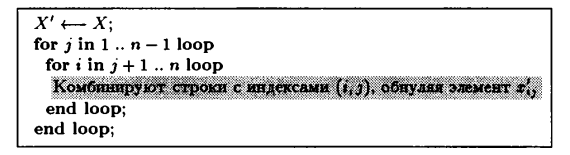
\includegraphics[height=18mm]{image1}
\end{wrapfigure}
как эти параллелограммы не имеют ни одной 
внутренней точки в $\mathbb {Z}^{2}$, то объединение их вершин 
является в точности квадратной сеткой $\mathbb {Z}^{2}$, и, 
следовательно, ${\vec{u},\vec{v}}$ образуют систему образующих $\mathbb {Z}^{2}$. 
Отсюда следует, что ${\vec{u},\vec{v}}$ является базисом $\mathbb {Z}^{2}$ и



%\lhead{\small\textit{Решение упражнений}}
%\rhead{403}

$|det(\vec{u},\vec{v})| = 1$ является числом, представляющим площадь параллелограмма (площадь треугольника равна половине площади параллелограмма) , что совпадает с формулой Пика.

\subparagraph{b.} Рассмотрим два приведения $\mathcal{P} \rightarrow \mathcal{P}'$ и $\mathcal{P} \rightarrow \mathcal{P}''$. Первое состоит в присоединении внутренней точки $\mathcal{P}$ к двум вершинам. Второе --- в присоединении двух вершин $\mathcal{P}$ так, чтобы треугольник $\mathcal{T}$, ограниченный таким образом, отвечал условиям пункта {\bf a} (см. рис. 1).

В первом случае получают многоугольник $\mathcal{P}'$ с характеристикой $(n',f')$, а во втором случае — многоугольник $\mathcal{P}''$ с характеристикой $(n'',f'')$, связанные отношениями:

\begin{equation*}
i' = i - 1,\;\;\; f' = f + 1,\;\;\; i'' = i,\;\;\; f'' = f - 1,
\end{equation*}

\begin{tabular}{ccl} 
площадь($\mathcal{T}$) = $\frac{1}{2}$,$\;\;$ площадь($\mathcal{P}$) &=& площадь($\mathcal{P}'$) + площадь($\mathcal{T}$) = \\
                                                       &=& площадь($\mathcal{P}''$) + площадь($\mathcal{T}$).
\end{tabular} 

\begin{figure}[h]
\center{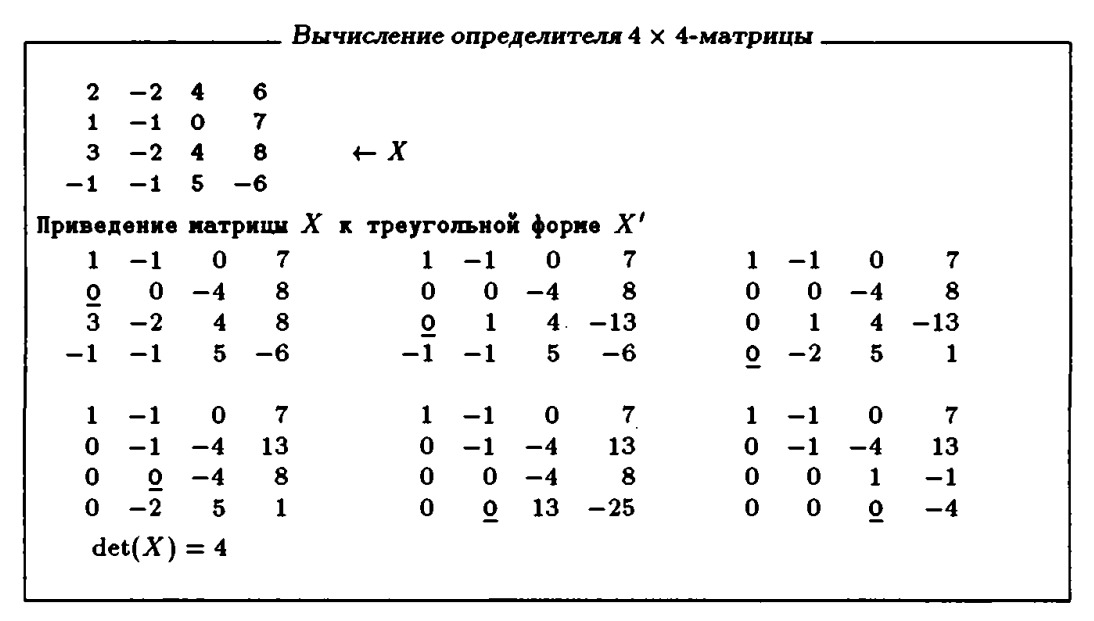
\includegraphics[width=75mm]{image2}}
\caption{Приведения многоугольника}
\end{figure}



\noindent Эти соотношения доказывают, что если формула Пика истинна для $\mathcal{P}'$ (соответственно для $\mathcal{P}''$), она истинна и для $\mathcal{P}$. Здесь был использован тот факт, что можно всегда применить одно из двух приведений, что позволяет доказать формулу Пика по индукции.

\paragraph{29. Теорема о ядре}

\subparagraph{а.} Пусть $b_{i} = a_{1}a_{2}\ldots a_{i-1}a_{i+1}\ldots a_{k}$. Тогда $b_{i}$ взаимно просты, следовательно, существуют такие $u_{1},\ldots,u_{k}$, что 1 = $u_{1}b_{1}+u_{2}b_{2}+\dots+u_{k}b_{k}$. Для $x \in M$ имеет место равенство:

\begin{equation}
x = u_{1}b_{1}x + u_{2}b_{2}x +\dots+ u_{k}b_{k}x, \text{и} x \in Ker_{M} a_{2} \Rightarrow b_{i}x \in Ker_{M} a_{i},
\end{equation}

\noindent откуда следует равенство $Ker_{M} a = Ker_{M} a_{1} + Ker_{M} a_{2} +\dots+ Ker_{M} a_{k}$.

С другой стороны, если $x_{i} \in Ker_{M} a_{i}$, то $u_{j}b_{j}x_{i} = 0$ для $j \neq i$. В силу свойства (8): $x_{i} = u_{i}b_{i}x_{i}$. Следовательно, соотношение $\sum_{i = 0}^{k}x_{i} = 0$ влечет $x_{j} = 0$ и то, что сумма прямая.



%\lhead{404}
%\rhead{\rm{III} \small\textit{Модули над кольцами главных идеалов}}

\subparagraph{с.} Имеют место равенства:

\begin{equation*}
(X - \lambda) \bullet e^{\lambda t}f = e^{\lambda t}\frac{df}{dt},\;\;\;\;\; (X - \lambda)^{n} \bullet e^{\lambda t}f = e^{\lambda t}\frac{d^{n}f}{dt^{n}},
\end{equation*}

\noindent и следовательно, $\rm{Ker}(X - \lambda)^{n} = \{R(t)e^{\lambda t} | R(t) \in C[t], deg(R) < n\}$.

\paragraph{31. Примарные модули над кольцом главных идеалов (задача)}

\subparagraph{a.} Из равенства $M = N \pi M$ следует:

\begin{equation*}
M = N \pi N + \pi^{2}M = N + \pi^{2}M =\dots= N + \pi^{3}M=\dots= N + \pi^{k}M = N,
\end{equation*}

\noindent что доказывает пункт ($i$).

$(ii) M = \sum_{i \in I}Ax_{i} + \pi M$, тогда в силу предыдущего результата
$M = \sum_{i \in I}Ax_{i}$ минимальность доказывается легко.

$(iii)$ Если $\pi$ не делит $a$, то $\pi^{k}$ и $a$ взаимно просты, тогда 1 является
линейной комбинацией $a$ и $\pi^{k}$, а так как $x$ обнуляется сразу значениями
$\pi^{k}$ и $a$, то $x = 0$. Получили противоречие.

$(iv)$ Заметим, что $\sum_{i}\mu_{i}x_{i} = 0 \Rightarrow \pi | \mu_{i}$. Действительно, используя
то, что сумма $\sum_{i \in I}A\pi x_{i}$ прямая, имеем: вышеприведенное равенство,
умноженное на $\pi$, дает $\mu_{i}\pi x_{i} = 0$. Так как $\pi x_{i} \neq 0$, то, в силу предыду-
щего результата, $\pi | \mu_{i}$.

В $M/\pi M$ равенство вида $\sum_{i \in I}\overline{\lambda_{i}}x_{i} = 0$, влечет равенства
$\sum_{i \in I}\lambda_{i}x_{i} = \pi\sum_{i \in I}\beta_{i}x_{i}$ и $\sum_{i \in I}(\lambda_{i} - \pi\beta_{i}) = 0$. В силу предыдущего
результата $\pi |\lambda_{i} - \pi\beta_{i} \Rightarrow \pi| \lambda_{i} \Rightarrow \overline{\lambda_{i}} = 0$, что и надо было доказать.

\subparagraph{b.} Запишем $\pi M$ в виде прямой суммы ненулевых однопорожденных
подмодулей:

\begin{equation}
\pi M = \bigoplus A\pi x_{i},\;\;\; где \pi x_{i} \neq 0.
\end{equation}

\noindent Тогда из пункта $(iv)$ вопроса {\bf a} известно, что множество $(\overline{x_{i}}_{i \in I})$ являет-
ся линейно независимым множеством векторного $A/\pi A$-пространства
$M/\pi M$. Дополним это множество до базиса $M/\pi M$. Пусть
$(\overline{x_{i}}_{i \in I}) \cup (\overline{z_{j}}_{j \in J})$ --- это базис.

Равенство (9) доказывает, что $\pi z_{j} \in \oplus_{i \in I}A\pi x_{i}$, т.е.
$\pi z_{j} = \sum_{i \in I}a_{ij}\pi x_{i}$. Положим $u_{j} = z_{j} - \sum_{i \in I}a_{ij}x_{i}$; множество
$(\overline{x_{i}}_{i \in I}) \cup (\overline{z_{j}}_{j \in J})$ будет всегда базисом $M/\pi M$, и в этом случае $u_{j}$ обну-
ляется $\pi: \pi u_{j} = 0$.
Докажем, что $M$ является прямой суммой следующих однопоро-
жденных модулей:

\begin{equation*}
M = \bigoplus Ax_{i} \oplus \bigoplus Au_{j}.
\end{equation*}



%\lhead{\small\textit{Решение упражнений}}
%\rhead{405}

\noindent Прежде всего, это множество является системой образующих, как это
было доказано во втором пункте $(ii)$ предыдущей задачи. Рассмотрим
соотношение $\sum_{i \in I}a_{i}x_{i} + \sum_{j \in J}b_{j}u_{j} = 0$. Приводя по модулю $\pi M$, полу-
чим $\pi\;|\;a_{i}$ и $\pi\;|\;b_{j}$. Из соотношения $\pi u_{j} = 0$ следует, что $b_{j}u_{j} = 0$. Если
записать $a_{i}$ в виде $a_{i} = \pi c_{i}$, получим $\sum_{i \in I}$, а так как сумма
в (9) прямая, то $c_{i}\pi x_{i} = a_{i}x_{i} = 0$, что и требовалось доказать.

\subparagraph{с.} Достаточно рассмотреть последовательность

\begin{equation*}
0 = \pi^{k}M \subset \pi^{k-1}M \subset\dots\subset \pi M \subset M
\end{equation*}

\noindent и заметить, что теорема истинна для подмодуля $\pi^{k-1}M$, который явля-
ется векторным $A/\pi A$-пространством. Простая индукция по $k$ доказы-
вает теорему.

\paragraph{32. Абелевы группы данного порядка $n$}

\subparagraph{а.} Пусть дана абелева группа $\Omega$ порядка $p^{r}$. Существует возраста-
ющая последовательность $(r_{1},r_{2},\ldots,r_{s})$ целых строго положительных
чисел, удовлетворяющих условию $r_{1} + r_{2} +\dots+ r_{s} = r$, и такая, что
$\Omega$ будет изоморфна $\mathbb {Z}_{p^{r_{1}}} \times \mathbb {Z}_{p^{r_{2}}} \times \dots \times \mathbb {Z}_{p^{r_{s}}}$, и эта последовательность
определяется единственным образом по структуре $\Omega$. Итак, достаточ-
но пронумеровать все такие последовательности (которые не зависят
от $p$). Для этого зафиксируем длину $s, 1 \leqslant s \leqslant r$, и рассмотрим лекси-
кографический порядок на возрастающих последовательностях целых
положительных чисел длины $s$ суммы $r$. Наименьшая последователь-
ность будет $(1,1,\ldots,1,r - (s - 1))$. «Хорошей» последовательностью в
лексикографическом порядке $(r_{1},r_{2},\ldots,r_{s})$ будет последовательность
$(r'_{1},r'_{2},\ldots,r'_{s})$, постоянная на местах $[i,s - 1]$ для определенного $i$:

\begin{equation}
(r_{1},r_{2},\ldots,r_{i-1},1 + r_{i},\ldots,1 + r_{i},r'_{s}), \\
\text{где} r_{1} +\dots+ r_{i-1} + (s-i)(1 + r_{i}) + r'_{s} = r.
\end{equation}

\noindent Из соотношения (10) следует:

\begin{equation*}
r'_{s} = r - (r_{1} + r_{2} +\dots+ r_{i-1}) - (s-i)(1 + r_{i}) = \\
       = (r_{i} + r_{i+1} +\dots+ r_{s}) - (s-i)(1 + r_{i}).
\end{equation*}

\noindent Чтобы сохранить возрастание, достаточно наложить условие $1 + r_{i} \leqslant r'_{s}$,
т.е.:

\begin{equation*}
(s - i + 1)(1 + r_{i}) \leqslant (r_{i} +\dots+ r_{s})
\end{equation*}

\noindent  Итак, «хорошей» будет последовательность (10), а индекс $i$ будет наи-
большим, удовлетворяющим условию (11). Это дает алгоритм 8.

\end{document}
